\chapter{Aerodynamics}
During the course of the midterm phase of the project, the aerodynamics department mainly focuses on advising the other departments quantitatively about configurations and design decisions, as most of the design options for aerodynamics have a direct influence on other subsystems. The department also worked on a first order drag estimation tool for the initial analyses of the concepts. The working principles of this tool are described here, as well as the verification and validation strategy for it. Other tools that are expected to be needed are also considered together with verification and validation strategies to accompany them.\\

\noindent Before any work on aerodynamics is done, however, the flow similarity factors; the Reynolds and mach number are determined. These parameters ensure that any aerodynamic properties under research can be taken at the correct flow conditions.\par
The Reynolds number is first calculated using \autoref{eq:reynoldsnumber}. Since the maximum operating altitude is defined as $20m$, the air density $\rho$ is set to $1.225kg/m^3$. The Reynolds number is given by \autoref{reynoldsnumber}. The flow velocity $V_{flow}$ is set as the maximum cruise velocity of $40km/h = 11.1m/s$. The characteristic length $l_{characteristic}$ would be different for each concept. It is however possible to currently set it at $1.89m$, the height of a 95th percentile person. This value is chosen due to the size constraints of the system under consideration and the fact that it has to carry a person. The dynamic viscosity $\mu$ is found in literature to be $1.818 * 10^{-5} kg/m s$ \cite{AirViscosity} at $20\degree C$. The resulting Reynolds number is used in the remainder of the midterm phase of the project. This can be adjusted after the final concept is selected in the trade-off to better represent the design. \par
The mach number is irrelevant for the flow similarity in this application as $M << 1$ and thus compressability effects can be neglected without major repercutions. In further research for aerodynamics, subsonic conditions are always used.

\begin{equation}
	Re = \frac{\rho * V_{flow} * L_{char}{\mu} = 1.414 * 10^6
	\label{eq:reynoldsnumber}
\end{equation}


\section{Design Options}



\section{Design Option Considerations}
This section first discusses some of the design considerations that came up in other departments' work. Most of these had an influence on aerodynamics that was desired to be further elaborated on.\\

\noindent The first aspect is that of encapsulation in the quadcopter concept. Aerodynamically speaking, this is a sensible consideration as certain forms of encapsulation have the potential to decrease the drag of the system substantialy. There is unfortunately no research available on the exact effects of encapsulation. Other systems, such as the VeloX from the Delft Human Power Team and the likes, have proven this to be a true statement however \webcite{HPTVeloX}.\par
Another aspect that is important to elaborate on, is the "icecream cone" shape in the third concept. The more technical term for this shape is a teardrop. Research on this mainly consists of hydrodynamic analyses in submarine design. Due to flow similarity, this research can be used to get a better understanding of the optimal shapes for this construction. The most important factor is the ratio of the overall length over the diameter. The optimal point for the drag coefficient is a length between 6 and 8 times the diameter of the teardrop shape \cite{ConeFlow2}.\par


\section{Drag Estimation Tool}
For performance calcultions, an important factor is the aerodynamic drag of the system. This section describes a tool used to make a first estimation of this parameter. This tool is also intended to be further expanded in later stages of this project to gain more insight on the aerodynamics of the system.\par
Since this is a first order estimation, this tool does not make use of flow simulation. It is chosen to use a simple set of geometries, for which the aerodynamic drag is well known and defined. The interaction between these parts is only simulated in a limited capacity.\\

\subsection{Model description}
A first step in creating a tool like described above, is to define the model. Before anything else, a reference frame is set up and a free body diagram is created. This free body diagram is shown in \autoref{fig:referenceframedrag}. As can be seen, only the drag is analysed by this tool. No other aerodynamic forces are taken into account in this design phase. The flow is also taken parallel to the x-axis, as is the drag force per its definition. All bodies will be described in this reference frame.

\begin{figure}[H]
	\centering
	\includegraphics[width=0.7\textwidth]{images/Reference_Frame.pdf}
	\caption{Frame of reference and free body diagram used by the drag estimation tool.}
	\label{fig:referenceframedrag}
\end{figure}

\noindent As stated earlier, the model uses a simplified set of geometrical shapes. This set consists of spheres, circular cylinders, cuboids, teardrops and flat plate disks. For each of these shapes, experimentally determinded values for the drag coefficient are found in literature for the appropriate Reynolds number. These values are presented in \autoref{tab:dragcoefficientes}. For the flat plate disk, the drag coefficient is taken on the low side of the given range, as this part is meant to simulate the rotor disks of the system and these are not solid disks. The value is fine-tuned during the validation stage for this tool.

\begin{table}[H]
\caption{Drag coefficients and the corresponding reference areas for each part used in the drag estimation tool. ($Re = 1.414 * 10^6$)}
\label{tab:dragcoefficientes}
\begin{tabular}{|l|l|l|}
\hline
\textbf{Part}   & \textbf{Drag coefficient}             & \textbf{Reference area} \\ \hline
Sphere          & 0.15 \cite{SphereFlow}                & Frontal Area            \\ \hline
Cylinder        & 0.4 \cite{CylinderFlow}               & Frontal Area            \\ \hline
Cuboid          & 0.8 \cite{CuboidFlow}                 & Frontal Area            \\ \hline
Teardrop        & 0.05 \cite{ConeFlow1\cite{ConeFlow2} 	& $\sqrt{Volume^2}$       \\ \hline
Flat Plate Disk & 0.005 \cite{FlatPlateFlow}            & Wetted Area             \\ \hline
Skin friction	& 0.02 \cite{FlatPlateFlow}				& Wetted Area			  \\ \hline
\end{tabular}
\end{table}

\noindent At the current time, the model only allows for placement with orientations parallel to the axes of the reference frame. The orientation vectors of the parts that are sensitive to this are defined in \autoref{fig:orientationdefinitiondrag}. This means that any parts that would be under an angle to the reference frame, are to be appropriately oriented within the limitations of the software. Any sphere shaped parts do not require orientation, as the sphere is symmetric in all directions. All cuboid parts have their sides parallel to the planes defined in the reference frame and their orientation is determined by dimensions in each axis direction.

\begin{figure}[H]
	\centering
	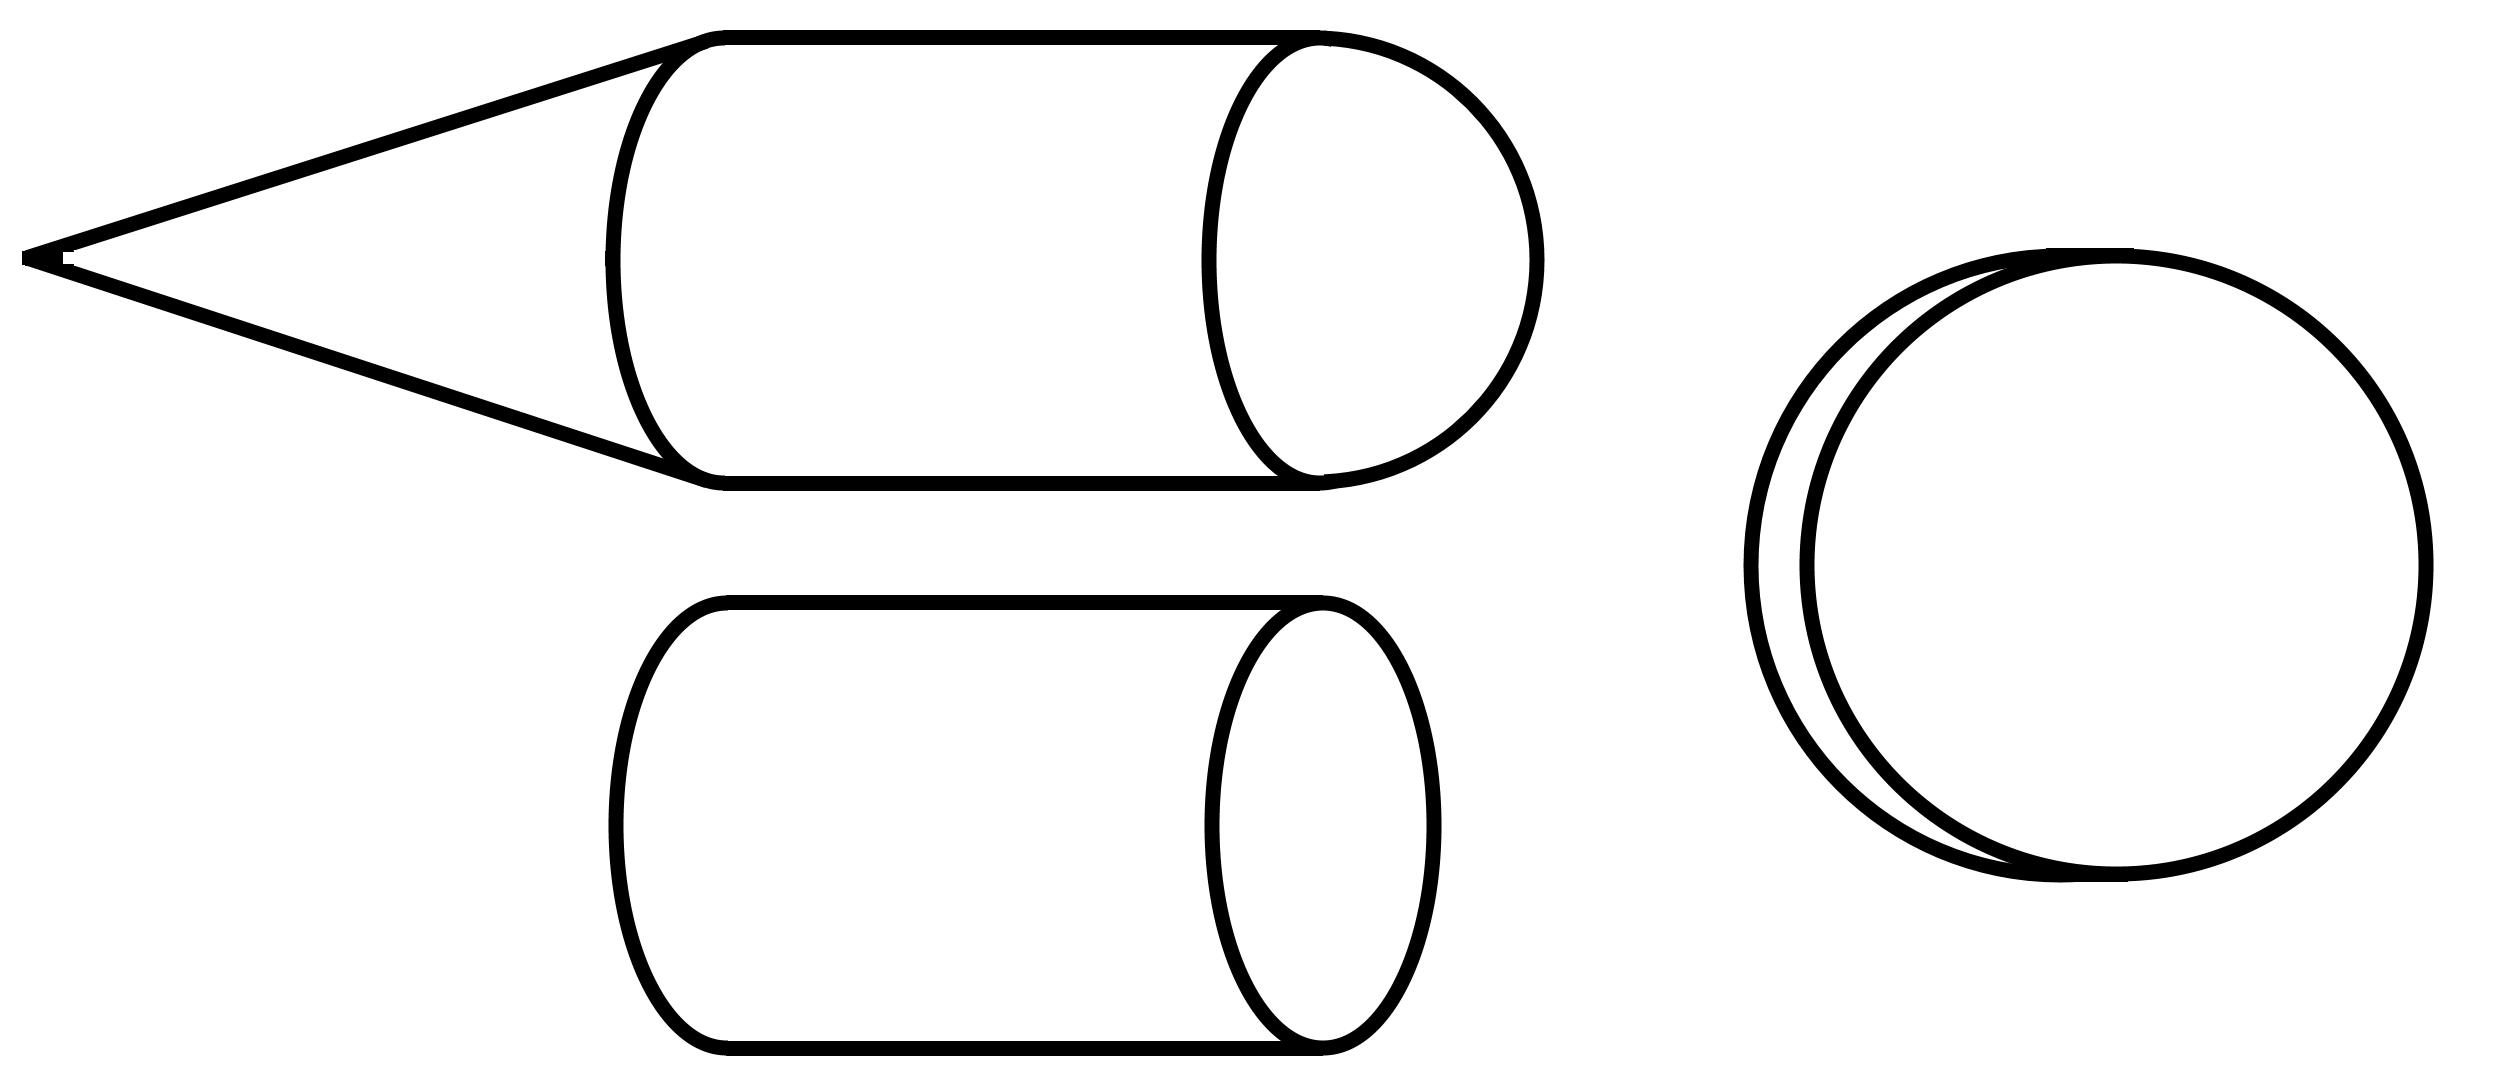
\includegraphics[width=0.5\textwidth]{images/Orientation_Definitions.pdf}
	\caption{Definition of the orientation vector of the teardrop, cylinder and flat plate disk respectively.}
	\label{fig:orientationdefinitiondrag}
\end{figure}

\noindent With all these parameters defined, the initial drag value of each part is calculated using the drag equation, given by \autoref{eq:dragequation}. These drag values are then corrected for the flow interaction between parts. Since this is hard to achieve without actual flow simulations, a simplified approach is taken. This approach consists of using a flow slowdown factor, which dictates the ratio $V/V_{flow}$. The ratio is taken from literature that investigates the wake of a cylinder \cite{WakeFlow}. It is assumed that these values hold for the other geometries under consideration, as wake flow research is not widely found for all geometries.

\begin{equation}
	D = \frac{1}{2} * \rho * V^2 * C_D * S_{ref}
	\label{eq:dragequation}
\end{equation}

\begin{equation}
	D_{pressure} = D_{total} - \frac{1}{2} * \rho * V_{flow}^2 * C_f * S_wet
	\label{eq:pressuredrag}
\end{equation}

The slowing down of the flow is not a constant over the distance behind an object, since the flow mixes again and velocities increase up to a certain new equilibrium far behind an object. To take this into account some values at different distances are defined from literature and later interpolated to find values at intermediate distances. In \autoref{fig:slowdowngraph} the flow slowdown is shown. The slowdown factor is only applied to an estimate of the pressure drag, which is defined in \autoref{eq:pressuredrag}. The value for the skin friction coefficient $C_f$ is taken as 0.025 \cite{FlatPlateFlow}. This is done to avoid completely negating a large object in the wake of a smaller object.

\begin{figure}[H]
	\centering
	\includegraphics[width=\textwidth]{images/Slowdown_graph.pdf}
	\caption{The flow slowdown behind a part. $L_char$ is defined here as the length, in the flow direction, of the part obstructing the flow.}
	\label{fig:orientationdefinitiondrag}
\end{figure}

After establishing the individual drag force for each component, the sum is taken to get an estimation of the overall system drag. This estimation clearly uses a few critical assumptions that are listed below. Due to these assumptions, a good validation strategy has to be established to check whether this method is valid for this type of analysis.

\begin{itemize}
	\item Incompressible flow is assumed.
	\item All geometry is simplified to a combination spheres, cylinders, cuboids, teardrops and flat plate disks.
	\item The drag of the flat plate disks is adjusted to be similar to a rotor disk, rather than a solid plate.
	\item Flow interaction of parts in the wake of another object is simulated by a flow slowdown factor.
	\item No other flow interaction between parts is taken into account.
	\item All parts are alligned with one or multiple of the axes.
\end{itemize}

\noindent This model is completely implemented in Python to form the drag estimation tool. All results are calculated with a precision of 3 significant digits, which will be further discussed in the verification results for this tool. This is a high enough degree of precision for this phase of the design and is considered adequate for further phases as well.

\subsection{Verification Strategy}
Verification consists

